\chapter{CVaR and Its Robust Formulation}

Despite its popularity as a measure of downside risk, VaR has received a fair amount of criticism \cite{capinski_risk,zhu,lim}. VaR for a diversified portfolio may exceed that for an investment in a single asset. Thus, one of the major limitations of VaR is the lack of sub-additivity in the case of general distributions. In accordance with this observation, VaR is not a coherent measure of risk as per the definition laid out by Artzner et al \cite{artzner}. Secondly, VaR does not provide any information on the size of losses in adverse scenarios \textit{i.e,} those beyond the confidence level ($1-\epsilon$). Additionally, VaR is non-convex and non-differentiable when incorporated into portfolio optimization problem. As a result, it becomes difficult to optimize VaR since global minimum may not exist. 

\section{Introduction}

Conditional Value-at-Risk (CVaR), introduced by Rockafellar and Uryasev \cite{rockafellar1,rockafellar2}, has addressed various concerns centred around VaR. For continuous distributions, CVaR is the expected loss conditioned on the loss outcomes exceeding VaR. For $\epsilon \in (0,1)$ , CVaR, at confidence level $1-\epsilon$, is defined as:
\begin{equation}
\label{eq:6.1}
CVaR_{\epsilon}(\mathbf{x}) \triangleq \frac{1}{\epsilon} \, \int \limits_{-\mathbf{r}^{\top}\mathbf{x} \geq VaR_{\epsilon}(\mathbf{x})} p(\mathbf{r})  d\mathbf{r}
\end{equation}
where $\mathbf{r}$ is the random return vector having probability density function $p(\mathbf{r})$ and $\mathbf{x}$ is the weight vector for a portfolio. In recent years, CVaR has emerged as a viable risk measure in portfolio optimization problems over its use in reducing downside risk. Since CVaR is a coherent risk measure, it follows the property of sub-additivity. Therefore, CVaR can be minimized through investment in a diversified portfolio. Unlike VaR, CVaR takes into consideration the impact of losses beyond the confidence level ($1-\epsilon$) \cite{capinski_risk}. Also, the minimization of CVaR is a convex optimization problem \cite{lim}.

Similar to Markowitz optimization and VaR minimization, there is an issue of lack of robustness in the classical framework of CVaR minimization. Computing CVaR requires the complete knowledge of the return distribution as argued by Zhu and Fukushima \cite{zhu}. They have addressed this shortcoming of the classical CVaR (henceforth, referred to as base-case CVaR) by proposing a new risk measure, namely, \textbf{Worst-Case CVaR (WCVaR)}. For a fixed weight vector $\mathbf{x}$, at confidence level $1-\epsilon$, WCVaR is defined as:
\begin{equation}
\label{eq:6.2}
WCVaR_{\epsilon}(\mathbf{x}) \triangleq \sup_{p(\mathbf{r}) \in \mathcal{P}}CVaR_{\epsilon}(\mathbf{x})
\end{equation}
where we assume that the density function $p(\mathbf{r})$ of returns belongs to a set $\mathcal{P}$ of probability distributions. The next section discusses coherent measures of risk that include both CVaR and WCVaR.

\section{Coherent Measures of Risk }
A risk measure $\rho$ is a mapping of random gain $X$ to a real value to represent the risk associated with $X$ quantitatively. In their seminal work on Coherent Measures of Risk, Artzner et al \cite{artzner} presented and justified following consistency rules for a risk measure $\rho$ to be coherent:
\begin{enumerate}
    \item{Monotonicity:}{$ \, X \leq Y \implies \rho (X) \geq \rho (Y) $}
    \item{Translation Invariance:}{ For any constant $m \in \mathcal{R}$, $ \rho (X + m) = \rho (X) + m $}
    \item{Positive Homogeneity:}{ For any positive constant $\lambda \geq 0$, $ \rho (\lambda X) = \lambda \rho (X) $}
    \item{Sub-additivity:}{ For any X and Y, $ \rho (X+Y) \leq \rho (X) + \rho(Y) $}
\end{enumerate}

It has been proved by Pflug \cite{pflug} and Acerbi and Tasche \cite{acerbi} that CVaR is a coherent measure of risk. Zhu and Fukushima \cite{zhu} have proved the coherence of WCVaR as a risk measure by analyzing it in terms of worst-case risk measure $\rho_{w}$:
\begin{equation}
\label{eq:6.3}
\rho_{w}(X) \triangleq \sup_{p(\mathbf{r}) \in \mathcal{P}} \rho (X)
\end{equation}


\section{Mathematical Formulations}
In this section, we discuss the mathematical formulations of the problems of optimizing CVaR along with WCVaR using mixture distribution uncertainty. We skip discussion on WCVaR formulations using box uncertainty set and ellipsoidal uncertainty set since they require a set of possible return distributions to be assumed so as to obtain bounds and scaling matrix respectively. However, our problem setup doesn't involve a set of return distributions since we make use of only market data (where return distribution is not known) and simulated data (where we generate a known return distribution).

\subsection {Minimizing Base-Case CVaR}
As proved by Rockafeller and Uryasev \cite{rockafellar1} , $CVaR_{\epsilon}(\mathbf{x})$, defined in equation (\ref{eq:6.1}), can be transformed into: 
\begin{equation}
\label{eq:6.4}
CVaR_{\epsilon}(\mathbf{x}) = \min_{\gamma \in \mathcal{R}^{n}} F_{\epsilon}(\mathbf{x},\gamma)
\end{equation}
where $n$ is number of assets in the portfolio and $F_{\epsilon}(\mathbf{x},\gamma)$ is defined as:
\begin{equation}
\label{eq:6.5}
 F_{\epsilon}(\mathbf{x},\gamma) \triangleq \gamma \, + \, \frac{1}{\epsilon} \, \int \limits_{\mathbf{r} \in \mathcal{R}^{n}} [-\mathbf{r}^{\top}\mathbf{x}-\gamma]^{+} p(\mathbf{r})  d\mathbf{r}
\end{equation}
In the above equation, $[t]^{+}=\max \{t,0\}$. The problem of approximation of the integral involved in the equation (\ref{eq:6.5}) can be dealt by sampling the probability distribution of $\mathbf{r}$ as per its density $p(\mathbf{r})$. Assuming there are S samples, $\{ \mathbf{r}_{1}, \mathbf{r}_{2}, .., \mathbf{r}_{i},..,\mathbf{r}_{S}\}$ for the return vector $\mathbf{r}$, $ F_{\epsilon}(\mathbf{x},\gamma)$ can be approximated as \cite{rockafellar1}:
\begin{equation}
\label{eq:6.6}
 F_{\epsilon}(\mathbf{x},\gamma) \approx \gamma \, + \, \frac{1}{S \, \epsilon} \, \sum_{i=1}^{S} [-\mathbf{r}_{i}^{\top}\mathbf{x}-\gamma]^{+} 
\end{equation}
In accordance with above approximation, the problem of minimization of classical CVaR, assuming no short-selling constraints, can be formulated as the following Linear Programming Problem (LLP) \cite{rockafellar1,zhu}:
\begin{equation}
\label{eq:6.7}
\begin{split}
& \min_{(\mathbf{x},\mathbf{u},\gamma,\theta)} \, \theta \, \, s.t. \\
& \mathbf{x}^{\top}\mathbf{1}=1, \mathbf{x} \geq \mathbf{0}, \\
& \gamma \, + \, \frac{1}{S \, \epsilon} \mathbf{1}^{\top}\mathbf{u} \leq \theta, \\
& u_{i} \geq -\mathbf{r}_{i}^{\top}\mathbf{x}-\gamma, \, u_{i} \geq 0, \, i=1,2,..,S. \\
\end{split}
\end{equation}
where the auxiliary vector $\mathbf{u} \in \mathcal{R}^S$ and $\theta$ is the auxiliary variable that is optimized to obtain the optimal value of the Base-Case CVaR.

\subsection {Minimizing Worst-Case CVaR using Mixture Distribution Uncertainty}
In this section, we describe the formulation of the optimization problem involving WCVaR by assuming that the return distribution belongs to a set of distributions comprising of all possible mixtures of some prior likelihood distributions \cite{zhu}. Mathematically, it is assumed that:
\begin{equation}
\label{eq:6.8}
p(\mathbf{r}) \in \mathcal{P}_{M} \triangleq \bigg\{ \sum_{j=1}^{l} \lambda_{j}p^{j}(\mathbf{r}) \, : \, \sum_{j=1}^{l}\lambda_{j}=1, \lambda_{j} \geq 0,j=1,2,..,l \bigg\}
\end{equation}
In the above equation, $p^{j}(\mathbf{r})$ denotes the $j^{th}$ likelihood distribution and $l$ is the number of the likelihood distributions. In accordance with above assumption of mixture distribution uncertainty (that involves $\mathcal{P}_{M}$ as a compact convex set) , $WCVaR_{\epsilon}(\mathbf{x})$, defined in equation (\ref{eq:6.2}), can be rewritten as the following min-max problem \cite{zhu}: 
\begin{equation}
\label{eq:6.9}
\begin{split}
& WCVaR_{\epsilon}(\mathbf{x}) = \min_{\alpha \in \mathcal{R}} \max_{j \in \mathcal{L} } F_{\epsilon}^{j}(\mathbf{x},\gamma) \, , \, \text{where} \\
& \mathcal{L} \triangleq \{ 1,2,..,l \} \\
& F_{\epsilon}^{j}(\mathbf{x},\gamma) \triangleq \gamma \, + \, \frac{1}{\epsilon} \, \int \limits_{\mathbf{r} \in \mathcal{R}^{n}} [-\mathbf{r}^{\top}\mathbf{x}-\gamma]^{+} p^{j}(\mathbf{r})  d\mathbf{r} \\
\end{split}
\end{equation}
Similar to the case involving classical CVaR in previous subsection, $F_{\epsilon}^{j}(\mathbf{x},\gamma)$ can be approximated via discrete sampling as:
\begin{equation}
\label{eq:6.10}
F_{\epsilon}^{j}(\mathbf{x},\gamma) \approx \gamma \, + \, \frac{1}{S_{j} \, \epsilon} \, \sum_{i=1}^{S_{j}} [-\mathbf{r}_{i,j}^{\top}\mathbf{x}-\gamma]^{+}
\end{equation}
In the above equation, $\mathbf{r}_{i,j}$ is the $i^{th}$ sample of the return with respect to $j^{th}$ likelihood distribution and $S_{j}$ is the number of samples corresponding to $j^{th}$ likelihood distribution. Accordingly, assuming non-negative weights, the problem of minimization of WCVaR over a feasible set of portfolios can be formulated as the following LLP \cite{zhu}:
\begin{equation}
\label{eq:6.11}
\begin{split}
& \min_{(\mathbf{x},\mathbf{u},\gamma,\theta)} \, \theta \, \, s.t. \\
& \mathbf{x}^{\top}\mathbf{1}=1, \mathbf{x} \geq \mathbf{0}, \\
& \gamma \, + \, \frac{1}{S_{j} \, \epsilon} \mathbf{1}^{\top}\mathbf{u}^{j} \leq \theta, \, \, j=1,2,..,l,\\
& u_{i}^{j} \geq -\mathbf{r}_{i,j}^{\top}\mathbf{x}-\gamma, \, u_{i}^{j} \geq 0, \, \, i=1,2,..,S_{j}, \, \, j=1,2,..,l. \\
\end{split}
\end{equation}
In the above equation, the auxiliary vector $\mathbf{u}=(\mathbf{u}^{1} ; \mathbf{u}^{2} ; .. ; \mathbf{u}^{l}) \in \mathcal{R}^{S}$ where $\displaystyle{S=\sum_{j=1}^{l}S_{j}}$ and $\theta$ is the auxiliary variable whose optimization yields the optimal value of the Worst-Case CVaR..

\section{Computational Results}

Similar to the computational analysis of robust methods in Markowitz optimization and VaR minimization, we perform empirical analysis of the Worst-Case CVaR  model vis-\`a-vis the Base-Case CVaR model, making use of the historical market data and simulated data. Taking into consideration the number of stocks $N$, the comparative study is conducted under two scenarios, namely, $N=31$ and $N=98$. These numbers represent the number of stocks in S\&P BSE 30 and S\&P BSE 100 indices, respectively.

For each scenario, we use the same three sets of data as used in the performance analysis of robust approaches in Chapters 3 and 5 \textit{i.e,} a set of historical market data comprising daily log-returns and two sets of simulated data. The first set of simulated data comprises of the number of sample returns matching the number of return instances of the historical market data, say $\zeta (<1000)$. On the other hand, the second set has a larger number of samples, namely, 1000.

During computation of the Base-Case CVaR model, $S$ in equation (\ref{eq:6.7}) is set equal to the number of return samples, \textit{i.e,} either $\zeta$ or $1000$, depending upon the set of data used. We perform computation of the Worst-Case CVaR model, as formulated in equation (\ref{eq:6.11}), for values of $l$ in $\{2,3,4,5\}$ by setting $\displaystyle{S_{j}=\frac{S}{l}}$ where $\displaystyle{j \in \{1,2,..,l \}}$. Note that $l=1$ yields the same case as the classical CVaR model. We do not include larger values of $l$ in the discussion on the empirical results since this leads to a great decrease in the sample size for the likelihood distributions.

We perform comparative analysis of the Worst-Case CVaR model with respect to the Base-Case CVaR model using the Sharpe Ratio of the constructed portfolios having confidence level greater than $90\%$, \textit{i.e,} $\epsilon \in (0,0.1)$. Similar to preceding chapters, for computing the Sharpe Ratio, we assume the annualized risk free rate equal to $6\%$. In the following subsections, we present the computational results for the two scenarios.

\subsection{Performance with $N=31$ Assets}



We begin with the analysis for $N=31$ assets, in the case of the historical market data having log-returns of the stocks comprising S\&P BSE 30. In Table \ref{avgtab:6.1}, we present the average Sharpe Ratio of the portfolios constructed for the Base-Case CVaR and Worst-Case CVaR models (denoted by $Avg. \, \, SR_{CVaR}$ and $Avg. \, \, SR_{WCVaR}$, respectively) for different values of $l$. \textbf{For this case as well as other cases, we choose the value of $l$ having maximum difference in the average Sharpe Ratio between the WCVaR and CVaR model.} Accordingly, we perform comparative study based on the plot of the Sharpe Ratio and tabulation of results for some selected values of $\epsilon$. The motivation behind following this kind of methodology for empirical analysis is to assess the practical viability of the robust technique over the classical method in CVaR minimization. In accordance with our methodology, the empirical results are presented for $l=2$ in Figure \ref{fig:6.1} and Table \ref{tab:6.1}. From Figure \ref{fig:6.1}, we observe that the Base-Case CVaR model performs better than its robust counterpart in terms of the Sharpe Ratio of the constructed portfolios having $\epsilon \in (0,0.1)$. Table \ref{tab:6.1} supports the above observation quantitatively.

\begin{table}[!h]
    \centering
    \captionsetup{justification=centering}

   \begin{tabular}{||c|c|c|c||}
   \hline
  
$l$ & $Avg. \, \, SR_{CVaR}$ & $Avg. \, \, SR_{WCVaR}$ & $Diff. \, \, in \, \, Avg. \, \, SR$ \\
  
  \hline
2 & 0.0856 & 0.0611 & -0.0245 \\
3 & 0.0856 & 0.0345 & -0.0511 \\
4 & 0.0856 & 0.0439 & -0.0417 \\
5 & 0.0856 & 0.031 & -0.0546 \\
  \hline
\end{tabular}
    \caption{Comparison of CVaR and WCVaR in case of Market Data (31 assets) for different values of $l$}
    \label{avgtab:6.1}
\end{table}

\begin{figure}[!h]
    \centering
   
    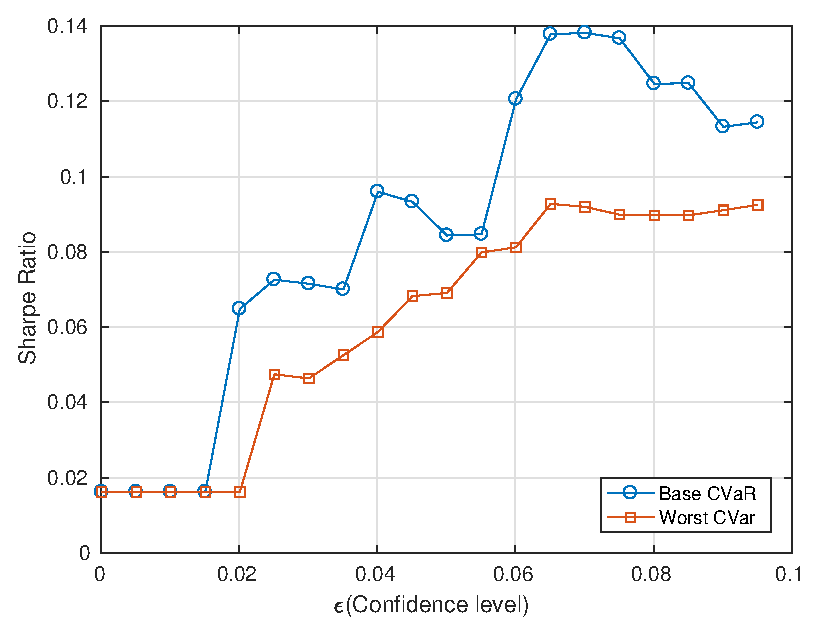
\includegraphics[height=7.0cm,width=0.7\textwidth]{CVaR/bse30_market/sr_cvar_2.eps}

   \caption{Sharpe ratio plot for CVaR and WCVaR in case of Market Data (31 assets) for $l=2$}
   \label{fig:6.1}
\end{figure}

\begin{table}[!h]
    \centering
    \captionsetup{justification=centering}

   \begin{tabular}{||c|c|c|c|c|c|c||}
   \hline
  
$\epsilon$ & $\mu_{CVaR}$ & $\sigma_{CVaR}$ & $\mu_{WCVaR}$ & $\sigma_{WCVaR}$ & $SR_{CVaR}$ & $SR_{WCVaR}$\\
  
  \hline
0.0001 & 0.000266 & 0.00661 & 0.000266 & 0.00661 & 0.0162 & 0.0162 \\
0.0201 & 0.000545 & 0.00595 & 0.000266 & 0.00661 & 0.0648 & 0.0162 \\
0.0401 & 0.000706 & 0.00569 & 0.000514 & 0.00603 & 0.096 & 0.0587 \\
0.0601 & 0.000832 & 0.00557 & 0.000645 & 0.00598 & 0.121 & 0.0812 \\
0.0801 & 0.000877 & 0.00576 & 0.000696 & 0.00597 & 0.125 & 0.0897 \\
  \hline
\end{tabular}
    \caption{Empirical Analysis of CVaR and WCVaR in case of Market Data (31 assets) for $l=2$}
    \label{tab:6.1}
\end{table}

On performing the simulation study with $\zeta$ samples, we draw an inference from Table \ref{avgtab:6.2} that the performance of the WCVaR model vis-\`a-vis the CVaR model is maximal for $l=5$. Similar to the methodology followed in the previous case, we present the relevant results for $l=5$ in Figure \ref{fig:6.2} and Table \ref{tab:6.2}. From the plot of the Sharpe Ratio in Figure \ref{fig:6.2}, we observe that the Worst-Case CVaR model starts outperforming the Base-Case CVaR model after $\epsilon$ crosses $0.05$ \textit{i.e,} incorporating robust optimization in CVaR minimization is advantageous in this case only for less conservative investors. We infer that the performance of the two models is almost equivalent, which is evident from Table \ref{tab:6.2} as well.

\begin{table}[!h]
    \centering
    \captionsetup{justification=centering}

   \begin{tabular}{||c|c|c|c||}
   \hline
  
$l$ & $Avg. \, \, SR_{CVaR}$ & $Avg. \, \, SR_{WCVaR}$ & $Diff. \, \, in \, \, Avg. \, \, SR$ \\
  
  \hline
2 & 0.103 & 0.102 & -0.000411 \\
3 & 0.103 & 0.103 & 0.000195 \\
4 & 0.103 & 0.104 & 0.00124 \\
5 & 0.103 & 0.106 & 0.00358 \\
  \hline
\end{tabular}
    \caption{Comparison of CVaR and WCVaR in case of Simulated Data with $\zeta$ samples (31 assets) for different values of $l$}
    \label{avgtab:6.2}
\end{table}

\begin{figure}[!h]
    \centering
   
    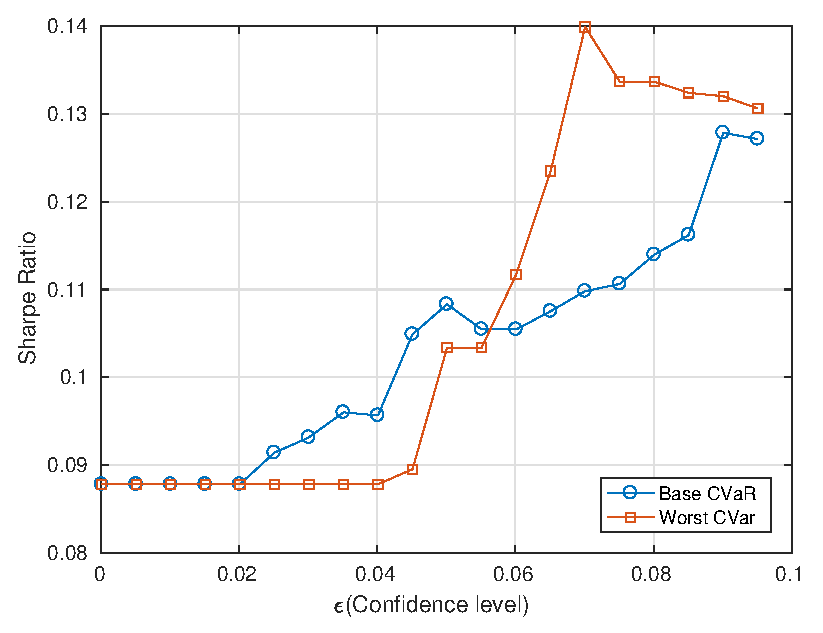
\includegraphics[height=7.0cm,width=0.7\textwidth]{CVaR/bse30_simulated/sr_exact_5.eps}

   \caption{Sharpe ratio plot for CVaR and WCVaR in case of Simulated Data with $\zeta$ samples (31 assets) for $l=5$}
   \label{fig:6.2}
\end{figure}

\begin{table}[!h]
    \centering
    \captionsetup{justification=centering}

   \begin{tabular}{||c|c|c|c|c|c|c||}
   \hline
  
$\epsilon$ & $\mu_{CVaR}$ & $\sigma_{CVaR}$ & $\mu_{WCVaR}$ & $\sigma_{WCVaR}$ & $SR_{CVaR}$ & $SR_{WCVaR}$\\
  
  \hline
0.0001 & 0.000675 & 0.00587 & 0.000675 & 0.00587 & 0.0878 & 0.0878 \\
0.0201 & 0.000675 & 0.00587 & 0.000675 & 0.00587 & 0.0878 & 0.0878 \\
0.0401 & 0.000694 & 0.00559 & 0.000675 & 0.00587 & 0.0957 & 0.0878 \\
0.0601 & 0.000731 & 0.00542 & 0.000838 & 0.00607 & 0.105 & 0.112 \\
0.0801 & 0.000776 & 0.00541 & 0.000889 & 0.00545 & 0.114 & 0.134 \\
  \hline
\end{tabular}
    \caption{Empirical Analysis of CVaR and WCVaR in case of Simulated Data with $\zeta$ samples (31 assets) for $l=5$}
    \label{tab:6.2}
\end{table}

The comparative analysis in terms of the average Sharpe Ratio with the number of simulated samples being $1000$ is presented in Table \ref{avgtab:6.3}. Accordingly, we select the value of $l$ equal to 4 and perform empirical study of the Base-Case CVaR and Worst-Case CVaR models, as presented in Figure \ref{fig:6.3} and Table \ref{tab:6.3}. It is difficult to draw any comparative inference from the Sharpe Ratio plot of the two models in Figure \ref{fig:6.3} since each outperforms the other in a different sub-interval of the range of $\epsilon$. The similar values of the Sharpe Ratio in Table \ref{tab:6.3} as well as the marginal difference in the average Sharpe Ratio for $l=4$ in Table \ref{avgtab:6.3} supports the claim of almost equivalent performance of the CVaR and WCVaR models in this case.

\begin{table}[!h]
    \centering
    \captionsetup{justification=centering}

   \begin{tabular}{||c|c|c|c||}
   \hline
  
$l$ & $Avg. \, \, SR_{CVaR}$ & $Avg. \, \, SR_{WCVaR}$ & $Diff. \, \, in \, \, Avg. \, \, SR$ \\
  
  \hline
2 & 0.0929 & 0.0967 & 0.00374 \\
3 & 0.0929 & 0.0945 & 0.00161 \\
4 & 0.0929 & 0.0969 & 0.00402 \\
5 & 0.0929 & 0.0954 & 0.00249 \\
  \hline
\end{tabular}
    \caption{Comparison of CVaR and WCVaR in case of Simulated Data with $1000$ samples (31 assets) for different values of $l$}
    \label{avgtab:6.3}
\end{table}

\begin{figure}[!h]
    \centering
   
    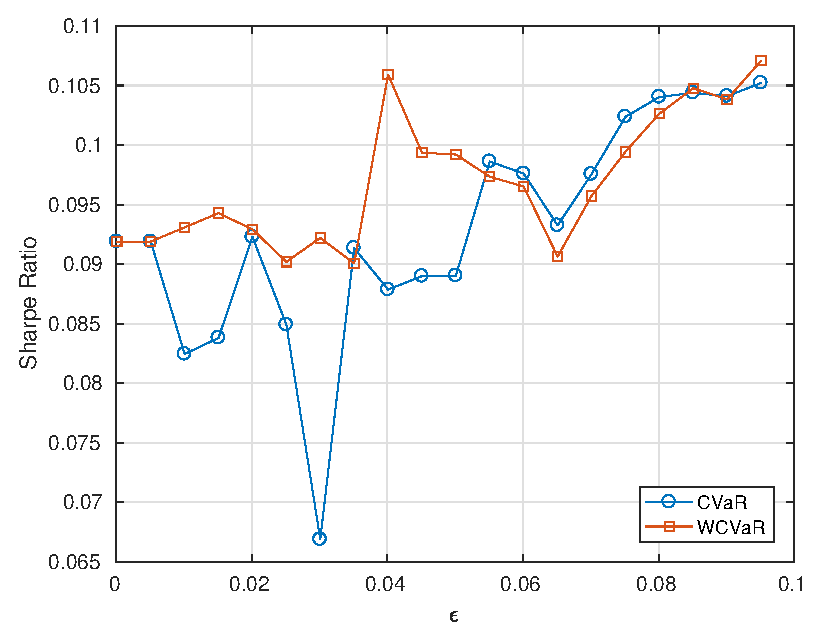
\includegraphics[height=7.0cm,width=0.7\textwidth]{CVaR/bse30_simulated/sr_1000_4.eps}

   \caption{Sharpe ratio plot for CVaR and WCVaR in case of Simulated Data with $1000$ samples (31 assets) for $l=4$}
   \label{fig:6.3}
\end{figure}

\begin{table}[!h]
    \centering
    \captionsetup{justification=centering}

   \begin{tabular}{||c|c|c|c|c|c|c||}
   \hline
  
$\epsilon$ & $\mu_{CVaR}$ & $\sigma_{CVaR}$ & $\mu_{WCVaR}$ & $\sigma_{WCVaR}$ & $SR_{CVaR}$ & $SR_{WCVaR}$\\
  
  \hline
0.0001 & 0.000677 & 0.00563 & 0.000677 & 0.00563 & 0.0919 & 0.0919 \\
0.0201 & 0.000658 & 0.0054 & 0.000661 & 0.0054 & 0.0923 & 0.0929 \\
0.0401 & 0.000629 & 0.00534 & 0.000722 & 0.00531 & 0.0879 & 0.106 \\
0.0601 & 0.00067 & 0.00523 & 0.000667 & 0.00526 & 0.0976 & 0.0965 \\
0.0801 & 0.000701 & 0.0052 & 0.000692 & 0.00519 & 0.104 & 0.103 \\
  \hline
\end{tabular}
    \caption{Empirical Analysis of CVaR and WCVaR in case of Simulated Data with $1000$ samples (31 assets) for $l=4$}
    \label{tab:6.3}
\end{table}

% \textbf{We infer a common observation from the three cases considered in the scenario involving less number of assets ($N=31$) \textit{i.e,} the WCVaR model performs at par with the CVaR model only in the case of simulated data. However, in the case of market data, the CVar model performs better than its robust counterpart.}


\subsection{Performance with $N=98$ Assets}

In this subsection, we consider the scenario involving $N=98$ assets. Table \ref{avgtab:6.4} summarizes the comparative results observed using the CVaR and WCVaR models on the historical market data (involving stocks comprising S\&P BSE 100). Since the difference between the average Sharpe Ratio of the WCVaR and CVaR models is maximum for $l=3$, so, we plot and tabulate the relevant results summarizing the empirical analysis of the two models for the same value of $l$ (Figure \ref{fig:6.4} and Table \ref{tab:6.4}). Similar to the corresponding case for the previous scenario, Figure \ref{fig:6.4} and Table \ref{tab:6.4} lead to an observation that the Base-Case CVaR model exhibits superior performance in comparison to the Worst-Case CVaR model, taking into consideration the Sharpe Ratio of the constructed portfolios as the performance measure. 

\begin{table}[!h]
    \centering
    \captionsetup{justification=centering}

   \begin{tabular}{||c|c|c|c||}
   \hline
  
$l$ & $Avg. \, \, SR_{CVaR}$ & $Avg. \, \, SR_{WCVaR}$ & $Diff. \, \, in \, \, Avg. \, \, SR$ \\
  
  \hline
2 & 0.121 & 0.102 & -0.0189 \\
3 & 0.121 & 0.105 & -0.0165 \\
4 & 0.121 & 0.0991 & -0.0219 \\
5 & 0.121 & 0.0927 & -0.0283 \\
  \hline
\end{tabular}
    \caption{Comparison of CVaR and WCVaR in case of Market Data (98 assets) for different values of $l$}
    \label{avgtab:6.4}
\end{table}

\begin{figure}[!h]
    \centering
   
    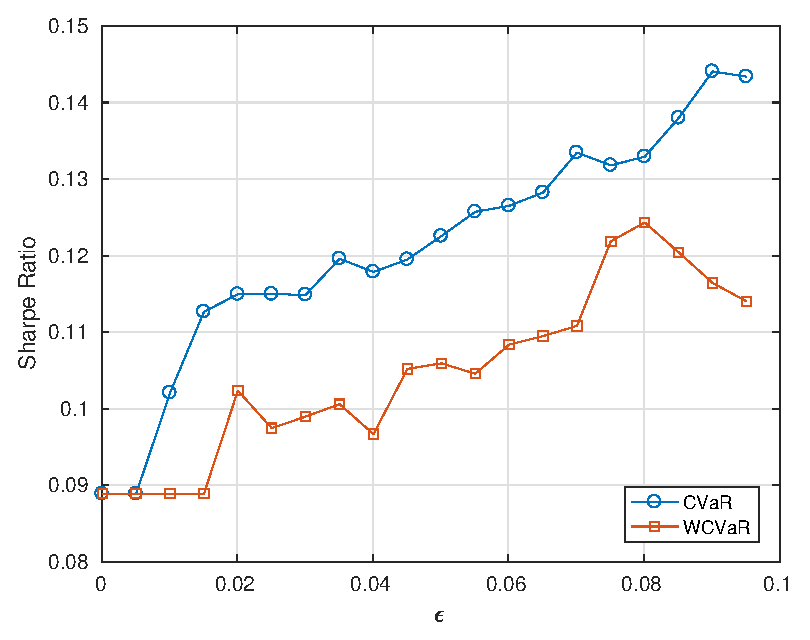
\includegraphics[height=7.0cm,width=0.7\textwidth]{CVaR/bse100_market/sr_cvar_3.eps}

   \caption{Sharpe ratio plot for CVaR and WCVaR in case of Market Data (98 assets) for $l=3$}
   \label{fig:6.4}
\end{figure}

\begin{table}[!h]
    \centering
    \captionsetup{justification=centering}

   \begin{tabular}{||c|c|c|c|c|c|c||}
   \hline
  
$\epsilon$ & $\mu_{CVaR}$ & $\sigma_{CVaR}$ & $\mu_{WCVaR}$ & $\sigma_{WCVaR}$ & $SR_{CVaR}$ & $SR_{WCVaR}$\\
  
  \hline
0.0001 & 0.000687 & 0.00593 & 0.000687 & 0.00593 & 0.0889 & 0.0889 \\
0.0201 & 0.000786 & 0.00544 & 0.000755 & 0.00582 & 0.115 & 0.102 \\
0.0401 & 0.00079 & 0.00535 & 0.000692 & 0.0055 & 0.118 & 0.0967 \\
0.0601 & 0.000839 & 0.00537 & 0.000738 & 0.00533 & 0.127 & 0.108 \\
0.0801 & 0.000847 & 0.00517 & 0.00082 & 0.00531 & 0.133 & 0.124 \\
  \hline
\end{tabular}
    \caption{Empirical Analysis of CVaR and WCVaR in case of Market Data (98 assets) for $l=3$}
    \label{tab:6.4}
\end{table}

Table \ref{avgtab:6.4} presents the comparison of the average Sharpe Ratio for the simulation study with $\zeta$ samples \textit{i.e,} same number of samples as that of log-returns of S\&P BSE 100 data. In accordance with the discussed methodology, we choose the value of $l$ equal to $4$ and present the empirical results in Figure \ref{fig:6.5} and Table \ref{tab:6.5}. From Figure \ref{fig:6.5}, we observe that the Worst-Case CVaR model almost outperforms the Base-Case CVaR model in terms of the Sharpe Ratio of the constructed portfolios having $\epsilon \in (0,0.1)$. From Table \ref{tab:6.5}, we can support this inference quantitatively by observing the greater Sharpe Ratio of the portfolios for the WCVaR model vis-\`a-vis the CVaR model. 

\begin{table}[!h]
    \centering
    \captionsetup{justification=centering}

   \begin{tabular}{||c|c|c|c||}
   \hline
  
$l$ & $Avg. \, \, SR_{CVaR}$ & $Avg. \, \, SR_{WCVaR}$ & $Diff. \, \, in \, \, Avg. \, \, SR$ \\
  
  \hline
2 & 0.0963 & 0.0978 & 0.00156 \\
3 & 0.0963 & 0.0968 & 0.000541 \\
4 & 0.0963 & 0.102 & 0.00581 \\
5 & 0.0963 & 0.0915 & -0.00479 \\
  \hline
\end{tabular}
    \caption{Comparison of CVaR and WCVaR in case of Simulated Data with $\zeta$ samples (98 assets) for different values of $l$}
    \label{avgtab:6.5}
\end{table}

\begin{figure}[!h]
    \centering
   
    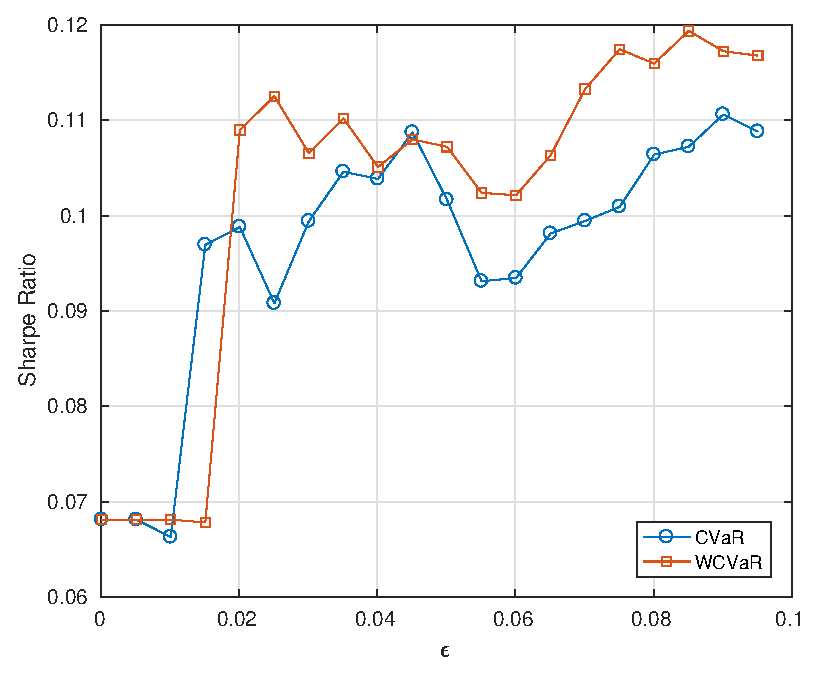
\includegraphics[height=7.0cm,width=0.7\textwidth]{CVaR/bse100_simulated/sr_exact_4.eps}

   \caption{Sharpe ratio plot for CVaR and WCVaR in case of Simulated Data with $\zeta$ samples (98 assets) for $l=4$}
   \label{fig:6.5}
\end{figure}

\begin{table}[!h]
    \centering
    \captionsetup{justification=centering}

   \begin{tabular}{||c|c|c|c|c|c|c||}
   \hline
  
$\epsilon$ & $\mu_{CVaR}$ & $\sigma_{CVaR}$ & $\mu_{WCVaR}$ & $\sigma_{WCVaR}$ & $SR_{CVaR}$ & $SR_{WCVaR}$\\
  
  \hline
0.0001 & 0.000554 & 0.00579 & 0.000554 & 0.00579 & 0.0681 & 0.0681 \\
0.0201 & 0.000703 & 0.0055 & 0.000755 & 0.00547 & 0.0988 & 0.109 \\
0.0401 & 0.000727 & 0.00546 & 0.000723 & 0.00536 & 0.104 & 0.105 \\
0.0601 & 0.000648 & 0.00522 & 0.000698 & 0.00527 & 0.0935 & 0.102 \\
0.0801 & 0.000706 & 0.00514 & 0.000768 & 0.00525 & 0.106 & 0.116 \\
  \hline
\end{tabular}
    \caption{Empirical Analysis of CVaR and WCVaR in case of Simulated Data with $\zeta$ samples (98 assets) for $l=4$}
    \label{tab:6.5}
\end{table}

Finally, the comparative analysis on the basis of the average Sharpe Ratio for the simulated data with $1000$ samples is presented in Table \ref{avgtab:6.6}. Accordingly, the results corresponding to the empirical study for $l=5$ are presented in Figure \ref{fig:6.6} and Table \ref{tab:6.6}. As observed from the plot of the Sharpe Ratio in Figure \ref{fig:6.6}, the Worst-Case CVaR model performs superior with respect to the Base-Case CVaR model almost entirely for $\epsilon \in (0,0.1)$. This observation is supported by the results presented in Table \ref{tab:6.6}.

\begin{table}[!h]
    \centering
    \captionsetup{justification=centering}

   \begin{tabular}{||c|c|c|c||}
   \hline
  
$l$ & $Avg. \, \, SR_{CVaR}$ & $Avg. \, \, SR_{WCVaR}$ & $Diff. \, \, in \, \, Avg. \, \, SR$ \\
  
  \hline
2 & 0.156 & 0.156 & -0.000382 \\
3 & 0.156 & 0.16 & 0.0037 \\
4 & 0.156 & 0.163 & 0.00667 \\
5 & 0.156 & 0.165 & 0.00868 \\
  \hline
\end{tabular}
    \caption{Comparison of CVaR and WCVaR in case of Simulated Data with $1000$ samples (98 assets) for different values of $l$}
    \label{avgtab:6.6}
\end{table}

\begin{figure}[!h]
    \centering
   
    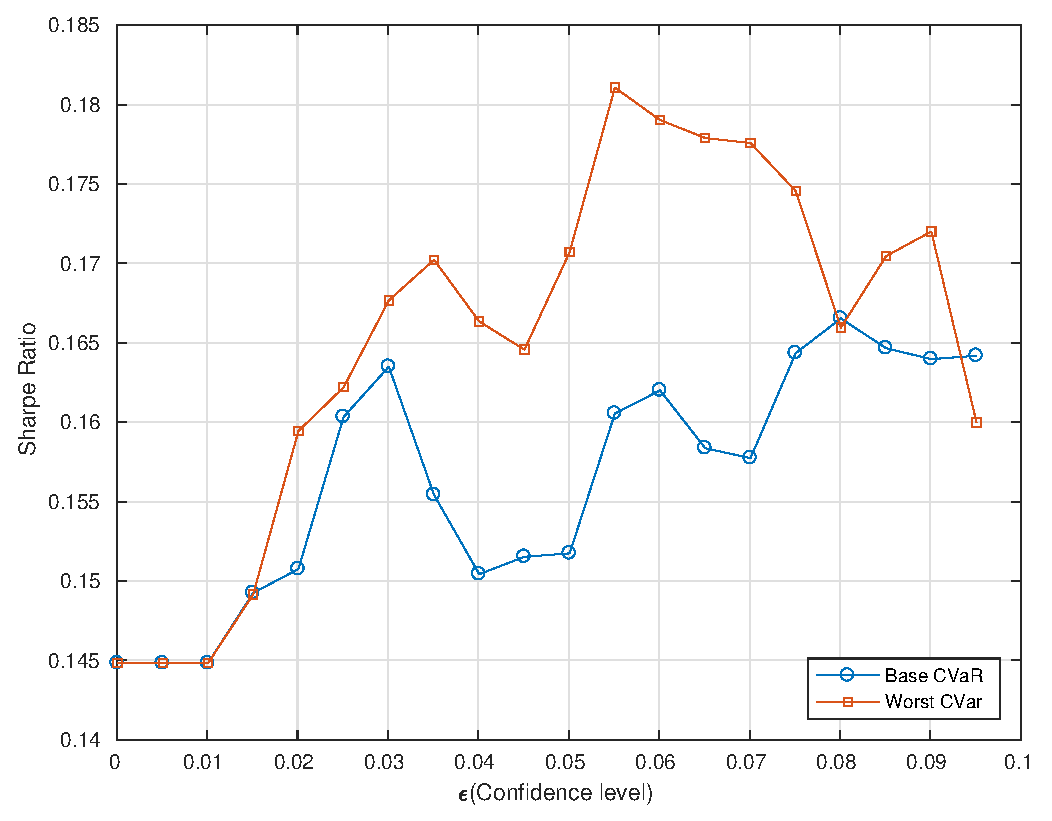
\includegraphics[height=7.0cm,width=0.7\textwidth]{CVaR/bse100_simulated/sr_1000_5.eps}

   \caption{Sharpe ratio plot for CVaR and WCVaR in case of Simulated Data with $1000$ samples (98 assets) for $l=5$}
   \label{fig:6.6}
\end{figure}

\begin{table}[!h]
    \centering
    \captionsetup{justification=centering}

   \begin{tabular}{||c|c|c|c|c|c|c||}
   \hline
  
$\epsilon$ & $\mu_{CVaR}$ & $\sigma_{CVaR}$ & $\mu_{WCVaR}$ & $\sigma_{WCVaR}$ & $SR_{CVaR}$ & $SR_{WCVaR}$\\
  
  \hline
0.0001 & 0.000935 & 0.00536 & 0.000935 & 0.00536 & 0.145 & 0.145 \\
0.0201 & 0.00097 & 0.00537 & 0.00101 & 0.00536 & 0.151 & 0.159 \\
0.0401 & 0.000927 & 0.0051 & 0.00104 & 0.00531 & 0.15 & 0.166 \\
0.0601 & 0.000963 & 0.00496 & 0.00106 & 0.00504 & 0.162 & 0.179 \\
0.0801 & 0.000974 & 0.00489 & 0.000981 & 0.00495 & 0.167 & 0.166 \\
  \hline
\end{tabular}
    \caption{Empirical Analysis of CVaR and WCVaR in case of Simulated Data with $1000$ samples (98 assets) for $l=5$}
    \label{tab:6.6}
\end{table}

% \textbf{A common inference that could be drawn from three cases considered in the scenario involving larger number of assets ($N=98$) is that the WCVaR model performs superior as compared to the CVaR model in the case of simulated data and vice-versa in the case of market data.}







